\chapter{Using SciLab}

\section{Basics}
When you first start SciLab you will see something like
\begin{verbatim}
                   ==========
                    scilab-2.7.2
        Copyright (C) 1989-2003 INRIA/ENPC
                    ==========



Startup execution:
  loading initial environment

-->
\end{verbatim}
The arrow ``$-$$-$$>$'' is the command prompt.  SciLab, like MatLab, is a command line interface to a mathematics programming environment.  To get started lets do a calculation.
\begin{verbatim}
3+(2+5*4)/11
\end{verbatim}
SciLab performs the calculation and displays the answer.
\begin{verbatim}
 ans  =

    5.
\end{verbatim}
Now lets define a simple variable.
\begin{verbatim}
a=2
\end{verbatim}
SciLab responds with
\begin{verbatim}
 a  =

    2.
\end{verbatim}
Notice anything similar?  The response is almost the same but ``ans'' has been replaced by the variable name ``a''.  In fact it is even more similar than that.  When no assignment (``name='') is given, SciLab automatically assigns the result to the variable ``ans''.  Try using it.
\begin{verbatim}
a*ans
\end{verbatim}
SciLab will tell you that ``ans'' is now 10.  Lets move on and define a matrix.  Type the following
\begin{verbatim}
  A=[1,2;3,4;5,6]
\end{verbatim}
and press enter. Commas are used to separate elements and semicolons are used to separate rows.  Note that you could also have entered ``A'' using the alternate notation
\begin{verbatim}
  A=[[1 2];[3 4];[5 6]]
\end{verbatim}
or even (command prompt shown so you won't think something is wrong when it automatically appears, also you do not need to space over like I do to enter the numbers, I just find it easier to read)
\begin{verbatim}
-->  A=[[1 2]
-->     [3 4]
-->     [5 6]]
\end{verbatim}
Thus spaces work like commas and returns work like semicolons.  In any case, SciLab should respond by showing you that it has created the matrix variable as follows
\begin{verbatim}
 A  =

!   1.    2. !
!   3.    4. !
!   5.    6. !
\end{verbatim}
The variable ``A'' is now defined and can be used.  For instance we might want to define ``B'' to be ``A+A''.  Do this by typing
\begin{verbatim}
  B=A+A
\end{verbatim}
SciLab will add the matrices and define ``B'' to be the result, showing you the answer.
\begin{verbatim}
 B  =

!   2.     4.  !
!   6.     8.  !
!   10.    12. !
\end{verbatim}
This mode is useful for doing simple calculations and testing output.  We will refer to it as the interactive mode.  Since SciLab has an interactive mode that is command driven, it is reasonable to assume it would have a programming interface (we will refer to it as the programming mode).  I will show the use of programming mode later.

\section{Programming}

Scilab is a Matlab look alike.  We will use Scilab as it is free and open source.  If you know one, you can figure the other out easily.

There are two basic ways to interact with Scilab: command line execution, and script files\footnote{Scilab distinguishes between directly executed files (.sce) and function libraries (.sci) which must be called by something else.  Matlab just uses M-files, a .m extension.}. Yes there are others such as compiled programs (MEX-files in Matlab), a GUI - Scicos (Simulink in Matlab), and several interfacing programs, but they are not relevant to us at the moment.  We will primarily be concerned with the use of script files, because they are the most helpful.  Command line execution is really just for quick operations and checking of segments of code.  Scilab syntax is a high level programming language that interacts with a series of numerical libraries (most notably LinPack\footnote{Linear Algebra Package}, EisPack\footnote{Eigen Systems Package, i.e. eigenvalues and eigenvectors, for basic systems, symmetric systems, generalized, and singular value decompositions.}, and BLAS\footnote{Basic Linear Algebra Subroutines, of which there are 3 levels: 1 is vector-vector operations, 2 is matrix-vector operations, and 3 is matrix-matrix operations.}).  Like most programming languages we have two types of programs that can be written.  A regular program, which is written as you would type commands on the command line, is the most basic type and is often the way you will start homework problems and other projects.  I am not going to try to be exhaustive, as the help files are quite nice (type ``help'' for a searchable help file or ``help command'' for help on some command (obviously you must replace command with the actual command you want help on).  Functions, which are sub-programs called by another program (even by other functions), are probably the most useful, as they allow you to extend the language by defining new operations.  One of the side goals of this book is for you to walk away with a basic familiarity of the tools that you can use to do a variety of tasks.  So how do you specify which you want?  You will get a regular program unless you start the script file with the command function.  The syntax is

\begin{verbatim}
  function [a,b,...,c]=name(x,y,..., z)
\end{verbatim}

Note you can return multiple values.  You also have several command structures: for, while, and if-elseif-else.  To see how these work let's make up a program.

\SciLab{Quadratic Function}{code:quadratic}{Scilab/quadratic.sci}

Now we want to run it.  Create the following script file in Scipad (Scilab's editor) then save and execute.

\SciLab{Graphing a Quadratic}{code:quadraticexec}{Scilab/runmyfunction.sce}

The resulting graph is

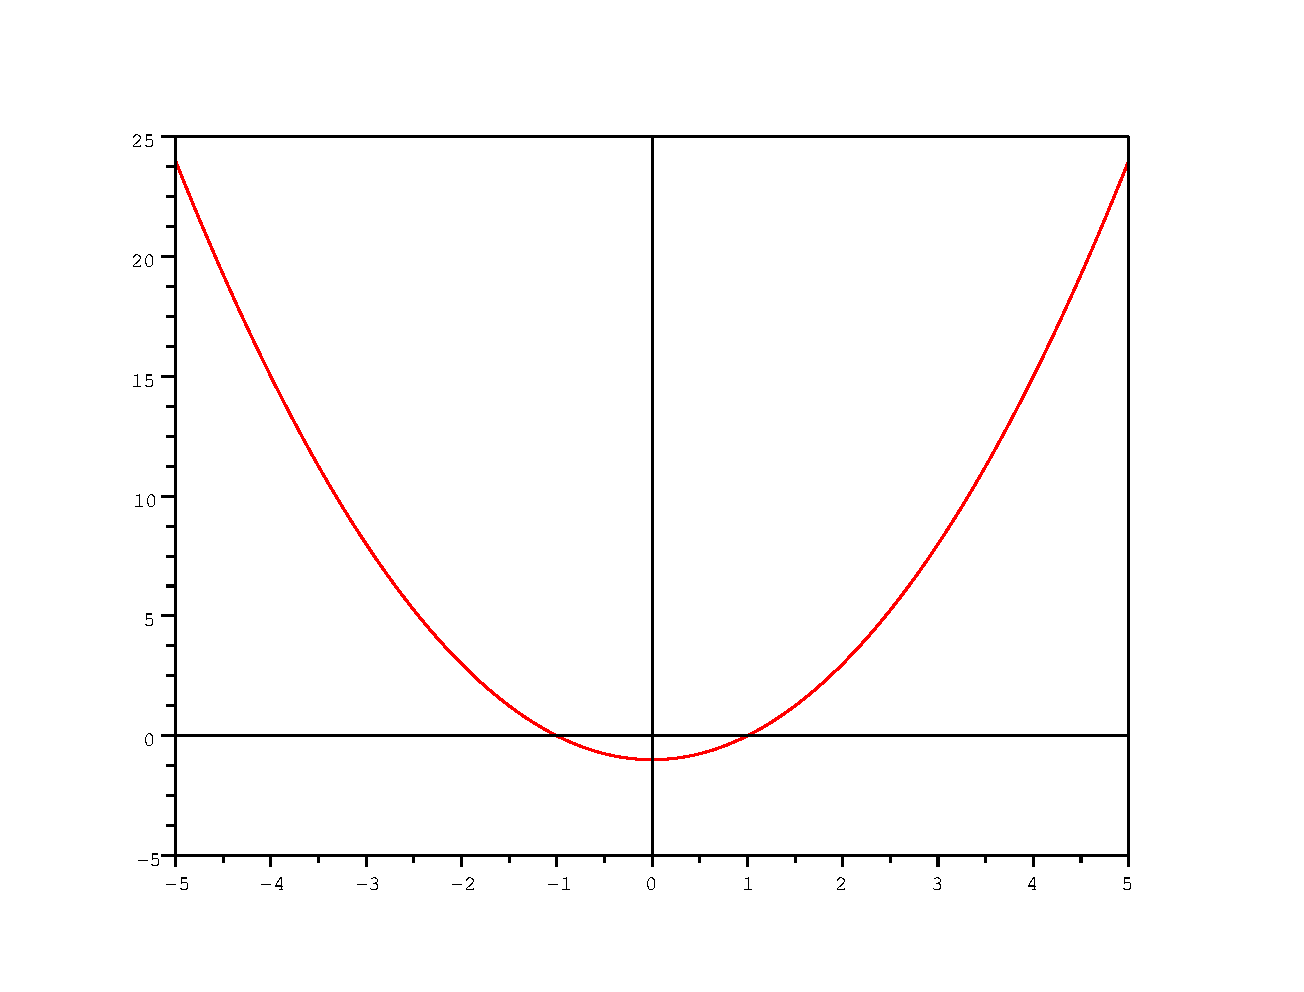
\includegraphics[width=\textwidth]{graphics/quadratic.eps}


\section{Scicos}

Scilab's graphical environment for evaluating block diagrams is called Scicos.  You can pull up the Scicos editor by typing
\begin{verbatim}
--> scicos
\end{verbatim}
A new window will open with a bunch of menus.  First we want to get our palettes so we can start adding things.  Click on the ``Palette'' menu and select ``Palettes''.  A menu will come up and you should select ``sources''.  Pull up the palettes again and select ``sinks''.  From the sources drag a ``sinusoid generator'' and a clock (needed to time the sampling of the sinusoid for the graph).  From the sinks drag the graph symbol in the lower left.  You can connect them by clicking on the arrows (source then sink) and a line will be dragged automatically.  By double clicking you can edit the parameters of a block.  We will leave the defaults for now.  Select the ``Simulate'' menu and then click on ``Setup''.  A window will pop up.  Change the ``Final integration time'' to 30 or it will run forever.  Now select the simulate menu again and click run.  A graph will appear and plot a sine function for 30 units.  If you did not change the final time it would just keep scrolling (a really annoying effect) and you would have to click ``Stop'' on the far right of the menu bar on the main Scicos window.

\begin{figure}
\caption{Scicos Sources}
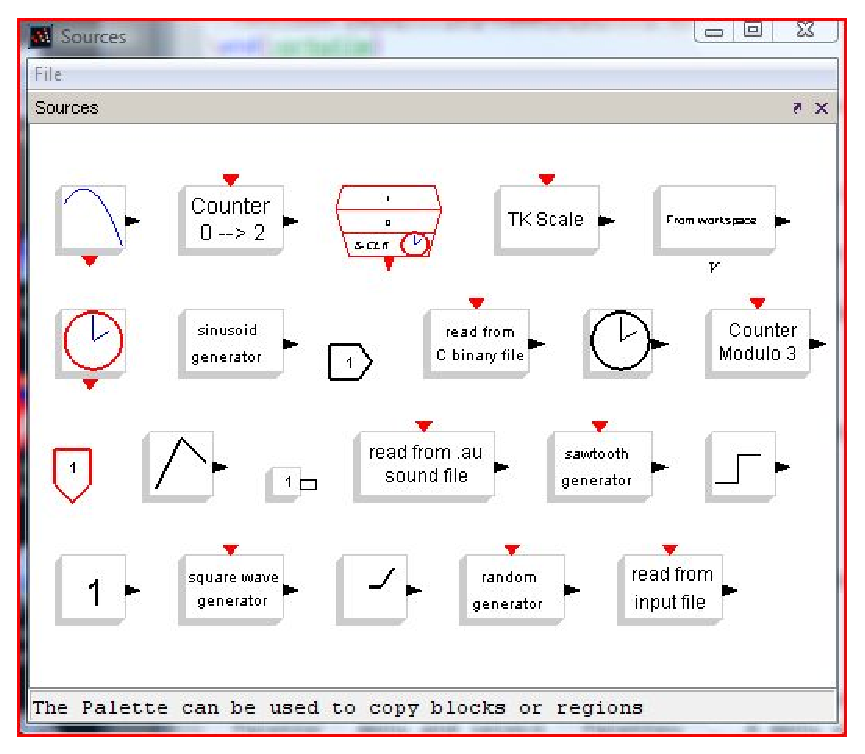
\includegraphics[width=.5\textwidth]{graphics/scicos_sources.eps}
\end{figure}

\begin{figure}
\caption{Scicos Sinks}
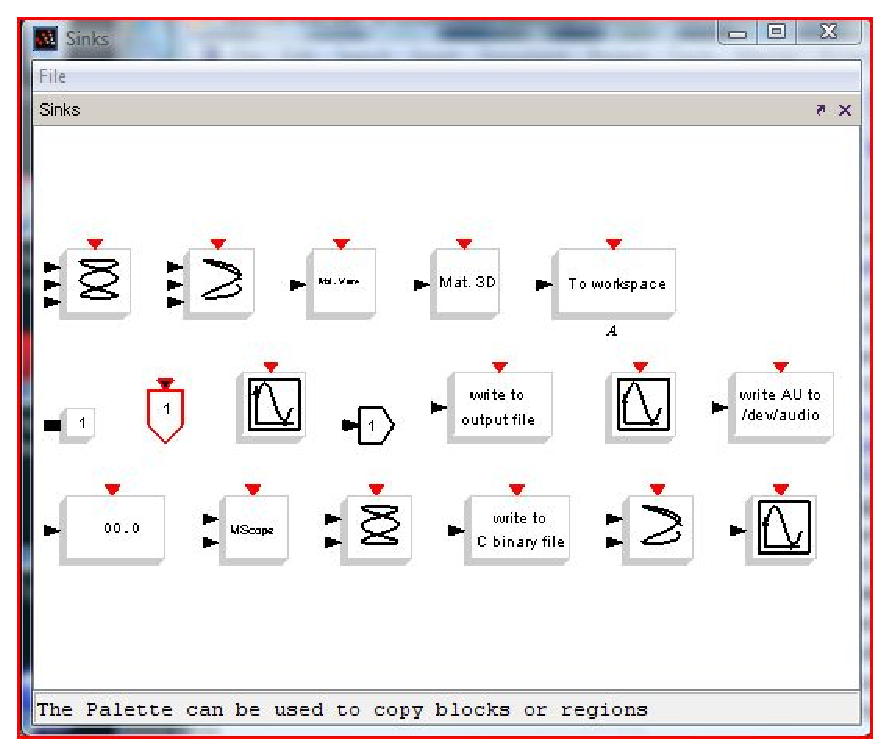
\includegraphics[width=.5\textwidth]{graphics/scicos_sinks.eps}
\end{figure}

\begin{figure}
\caption{Scicos Integration Model of Disease}
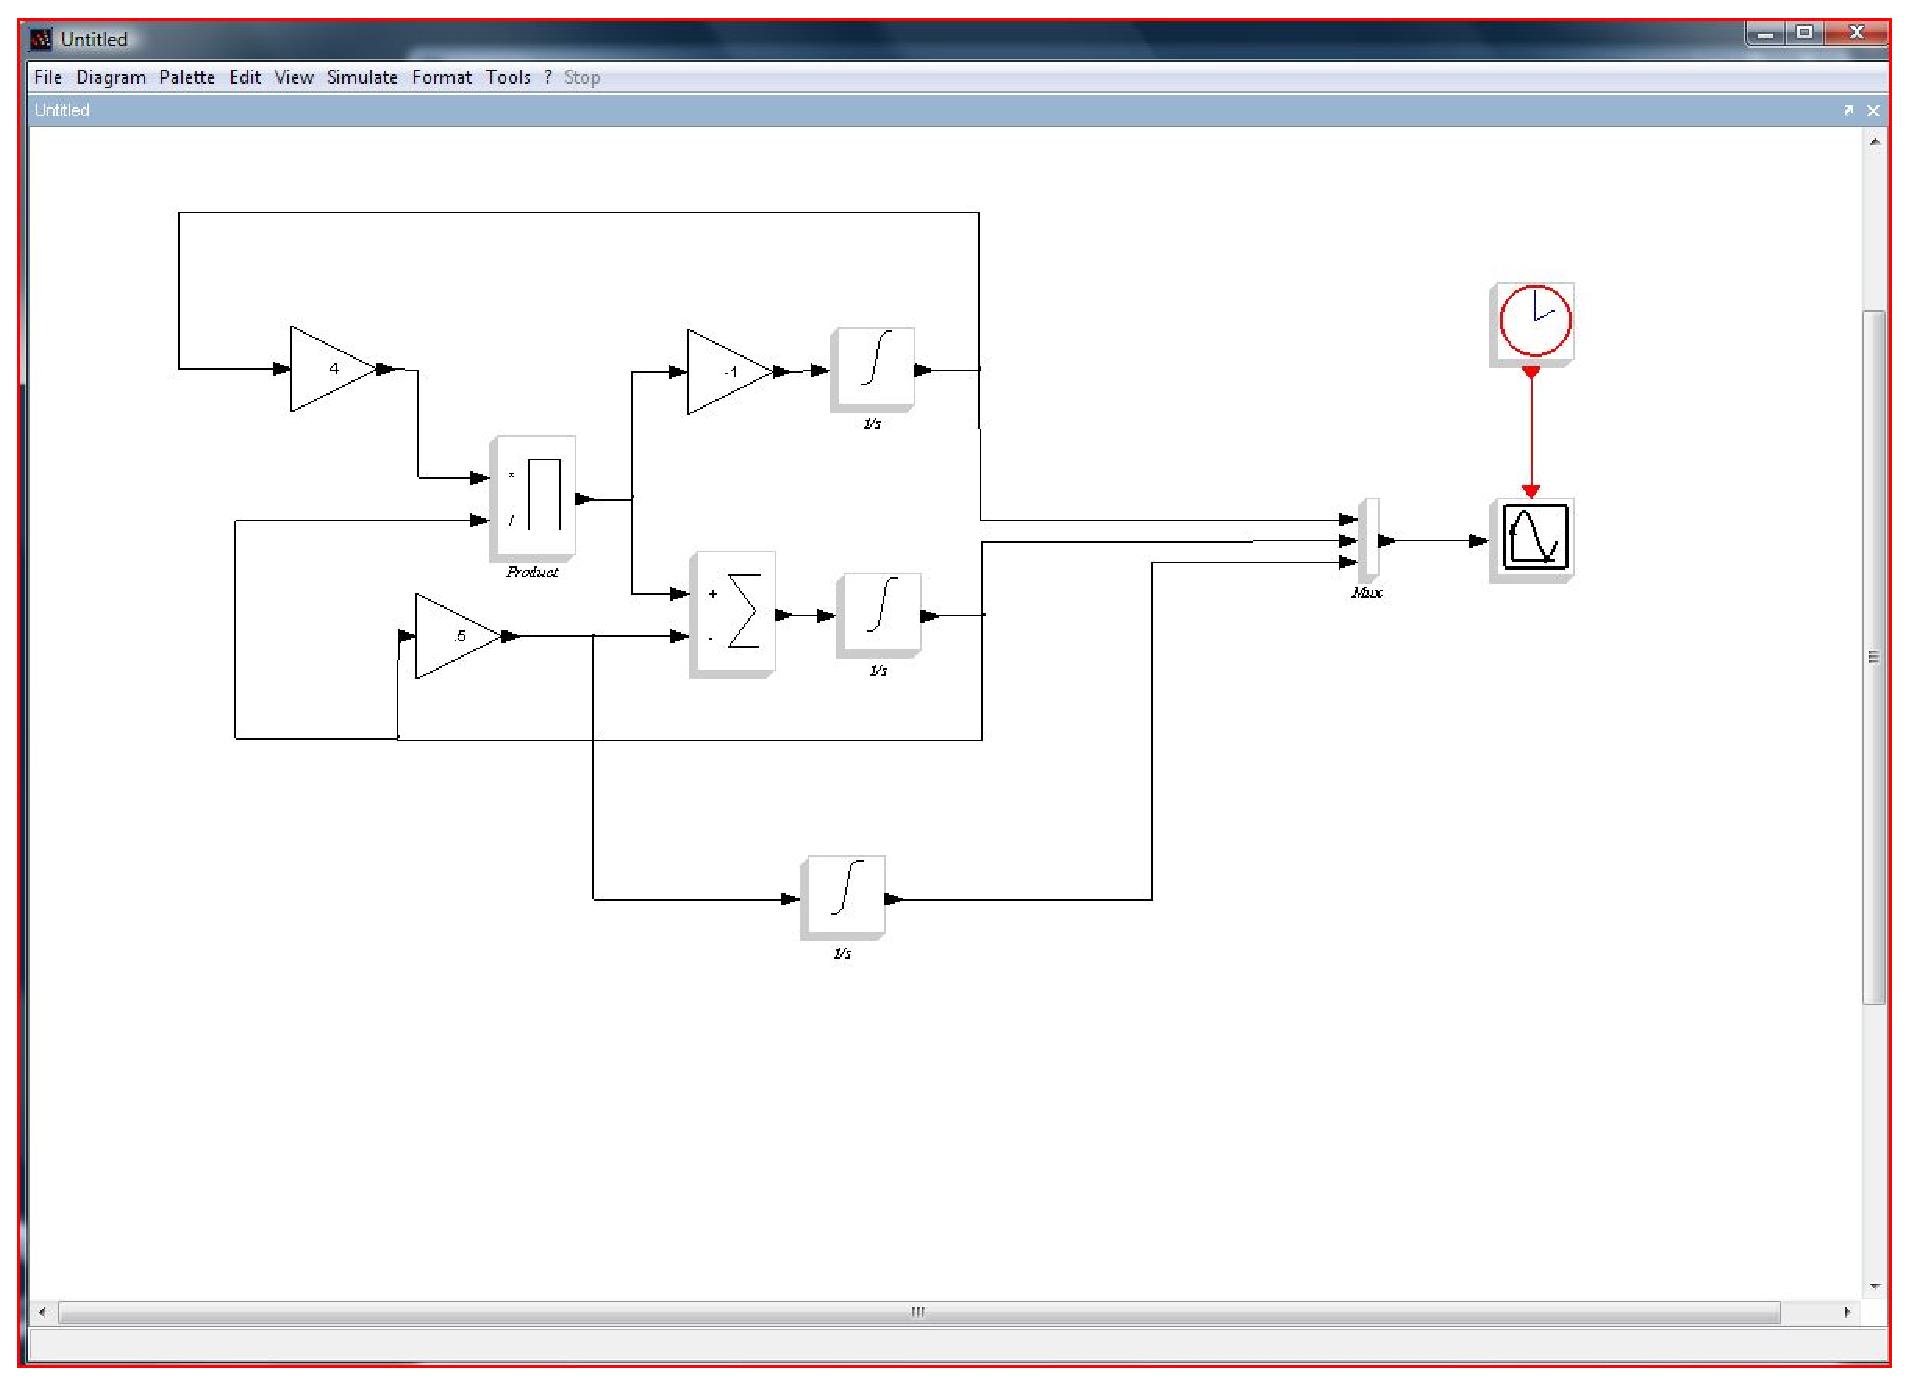
\includegraphics[width=\textwidth]{graphics/scicos_disease.eps}
\end{figure}

\begin{figure}
\caption{Scicos Plot of Disease Spread}
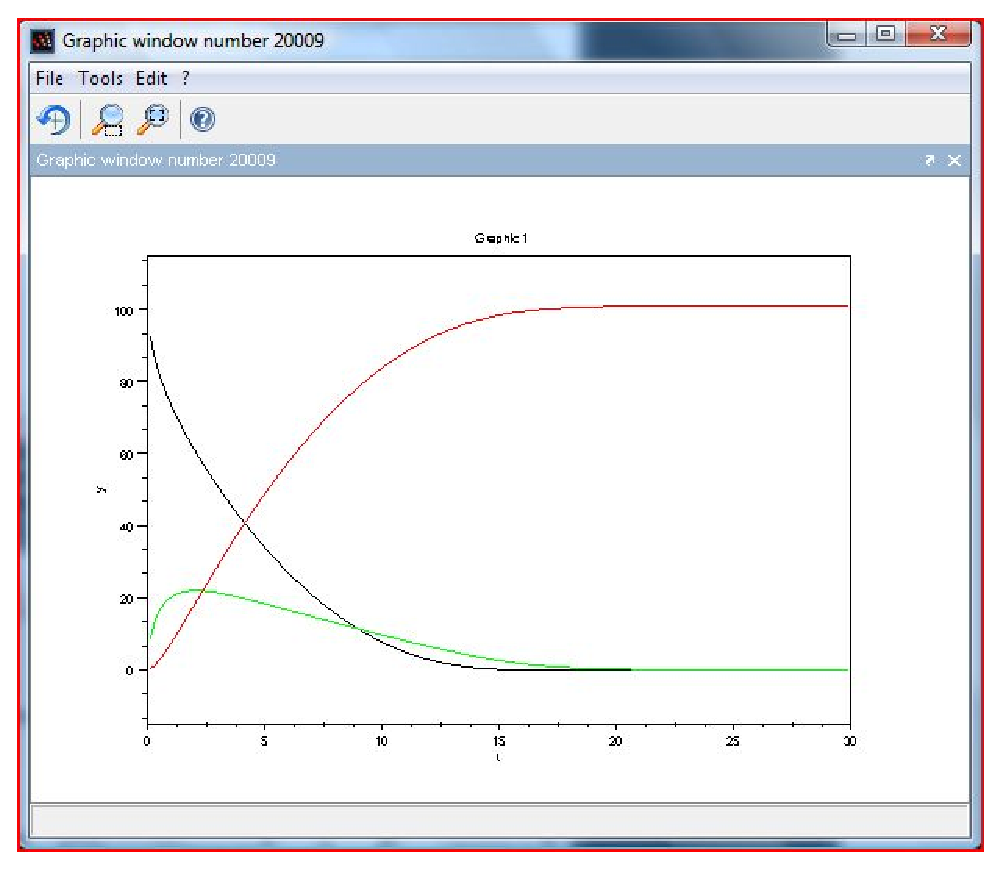
\includegraphics[width=\textwidth]{graphics/scicos_plot.eps}
\end{figure}

